

%ei varmaan saa olla kymy
\subsubsection{React Yleisesti}






% https://github.com/facebook/react/blob/main/README.md
% https://github.com/facebook/react/blob/f74c5ccf9469d3389ce3a1ee3b54988049e235f7/README.md
% https://www.infoq.com/news/2013/06/facebook-react/
% molemmat siteerattu 27.5.24

%https://opensource.fb.com/projects/react/
% 12.6

% https://react.dev/
% 30.5


%https://www.statista.com/statistics/1124699/worldwide-developer-survey-most-used-frameworks-web/
%yksi käytetyimmistä työkaluista 
% 30.5





React on Metan ylläpitämä avoimeen lähdekoodiin perustuva javascript kirjasto,
joka on suunniteltu reaktiivisien käyttöliittymien kehittämiseen\labcite{react24a}
React kannustaa kehittäjiä rakentamaan sovelluksia uudelleenkäytettävien komponenttien avulla.
Jokainen komponentti sisältää oman rakenteensa, tyylinsä ja käyttäytymisensä, joka tekee niistä helposti siirrettävän ja uudelleenkäytettävän.\labcite{react24a}
Komponenteista voidaan sitten koota monimutkaisia käyttöliittymimä. 
\medskip


Komponentit voidaan kirjoitetaa JSX syntaksilla, joka mahdollistaa HTML tyylisen kirjoituksen JavaScriptin sekaan.
Tämä tekee React:ista helppo luettavan, ymmärrettävän ja opittavan, joka on auttanut nostamaan reactin suosiota yhteen maailman käytetyimmistä käyttöliittymä työkaluista.\labcite{statista23}
\medskip









\subsubsection{JSX}





%https://react.dev/learn/writing-markup-with-jsx
%https://facebook.github.io/jsx/ 

% jsx = js xml
% https://medium.com/@sjarancio/what-is-jsx-e3dda0af3490

%transpilation
% https://www.scholarhat.com/tutorial/react/getting-started-with-jsx
% https://www.typescriptlang.org/docs/handbook/jsx.html

% kaikki viitattu 27.5







%html koodia uusiks syntaxia?
JSX (eng javascript XML) on sytaksi jatke javascriptille, joka antaa kehittäjän kirjoittaa HTML tyylistä syntaksia javascriptin sekaan, tekien koodista yksinkertaisempaa ja helpompaa ymmärtää. \labcite{Stephen21}
% suora sitaatti https://facebook.github.io/jsx/ 
JSX ei ole ECMAscript standardissa, joten selaimet eivät osaa tulkita sitä, vaan JSX se on suunniteltu transpiloitavaksi johonkin ECMAscript standardia toteuttavalle kielelle.\labcite{Facebook22}
\medskip

%muuttuja vois vaihtaa. johonkin toiseen suomalaiseen sanaan
Kuvassa \nextImageCount{} luodaan muuttuja helloWorld, jolle annetaan arvoksi HTML "p"{} elementti, jossa teksti "Hello, World!"{}.
% koko juttu uusiks ja paremmin kirjoitettua
Muuttujien arvot voidaan kirjoittaa HTML tyylillä, tekien monimutkaisten elementtien rakentamisesta yksinkertaista.
\medskip

\bigskip
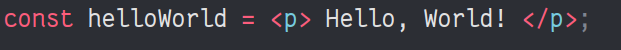
\includegraphics[width=10cm]{src/public/oppar/pure_jsx_example.png}\\
Kuva \getImgCount {}. esimerki JSX syntaxista
\medskip


Kuvassa \nextImageCount{} on kuvan \theimgCounter{} helloworld muuttuja, joka on käännetty natiiviksi JavaScriptiksi babel kääntäjää käyttäen. \labcite{babel24}
Tämä antaa selaimille mahdollisuuden suorittaa koodia, joka on alkuperin kirjoitettu JSX syntaksilla.
%jotain lisää tekstiä
\medskip


\bigskip
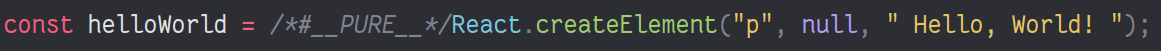
\includegraphics[width=15cm]{src/public/oppar/transpiled_jsx_example.png}\\
Kuva \getImgCount {}. Kuvan \prevImageCount{} JSX transpiloitu JavaScriptiin
\medskip





\subsubsection{Komponentit}




% kolmas kappale pitää korjata 
% kapale ennen kuvaa tarvitsee lisää sanaa


% komponentti joka voi renderöidä toisen komponentin. tämä jatkuu siihen asti että päästään natiiveihin html elementteihin jotka selain osaa tulkita
%https://react.dev/learn/your-first-component


Komponentti on oma pieni kokoonpano, joka sisältää sen ulkonäön ja käyttäytymisen.
Komponentit ovat olennainen rakennusosa React sovelluksissa. Reactissa Komponentit voivat olla tilallisia tai tilattomia. 
\medskip

%
Tilaton komponentti ei sisällä omaa tilaa. 
niiden pää tarkoitus on renderöidä käyttöliittymää niille annettujen propertyjen perusteella.
Tilattomat komponentit on helpompi kirjoittaa ja testata verrattuna tilalliseen komponenttiin, 
sillä niissä ei ole sivu efektejä eikä niiden käyttäntö tai ulkonäkö vaihdu sisäisen tilan takia.\labcite{Phuoc23}
\medskip


Tilallinen komponentti tarkoittaa komponenttia, joka sisältää oman tilan ja on vastuussa sen hallinnoinnista ja päivittämisestä.
%melkein kokonaan vaihtoon
Tilalliset komponentit ovat hyvä silloin kun pitää säilyttää käyttöliittymässä dataa ajanmyötä kuten form inputs tai datan hakua.\labcite{Phuoc23}\\
\medskip


%tarvitsee ainakin yhden lausekkeen lisää
React tukee kahta tapaa luoda komponentteja. Luokkakomponentti ja funktiokomponentti.\citemissing
Kuvassa \nextImageCount {} on esimerkki tilallisesta funktiokomponentista.
%molemmat toimii jotain lorem
\medskip


\bigskip
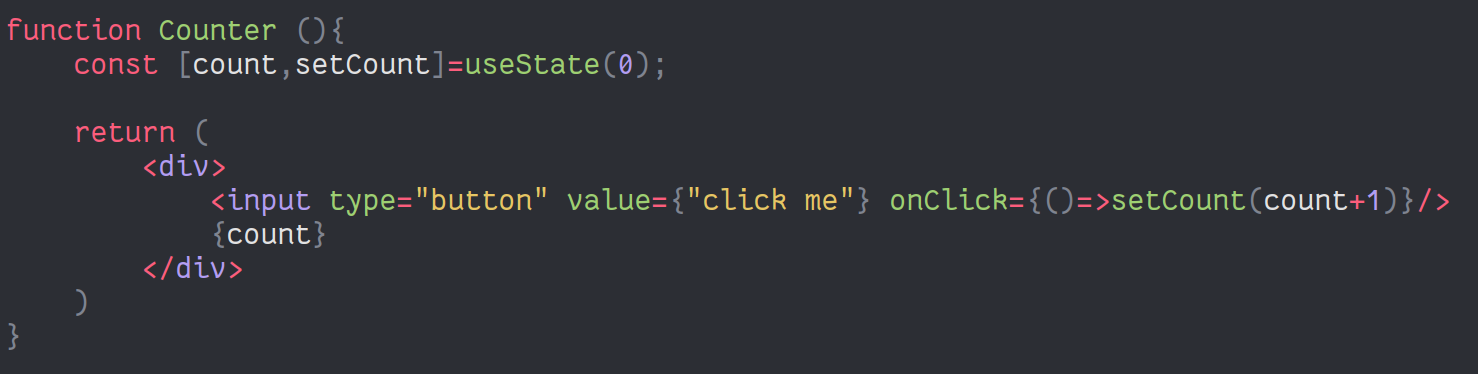
\includegraphics[width=15cm]{src/public/oppar/function_component.png}\\
Kuva \getImgCount{}. kuvakaappaus React komponentista
\medskip

Kuvaassa teemmme funktio komponentin laskija, joka seuraa kuinka monta kertaa nappia on painettu.
Kunktio palauttaa komponentin ulkonäön, joka on määritetty JSX syntaxilla.
Komponentissa on myös useState "hook"{}, joka kuvaistaa komponentin tilan, tätä käytten komponentti pystyy säilyttämään dataa ja päivittämään itsensä kun sen sisäinen tila muuttuu.
\medskip

%kirjoita uusiks
Komponentteja voidaan myös määrittää luokkakomponentti tyylillä. Mutta React on kehottaa käyttää funktiokomponentteja tulevaisuudessa. \labcite{react24c}
Kuva \nextImageCount {} on sama laskukomponentti kuin kuva \theimgCounter{} mutta kirjoitettu luokkakomponentti tyylillä. 
\medskip
\bigskip


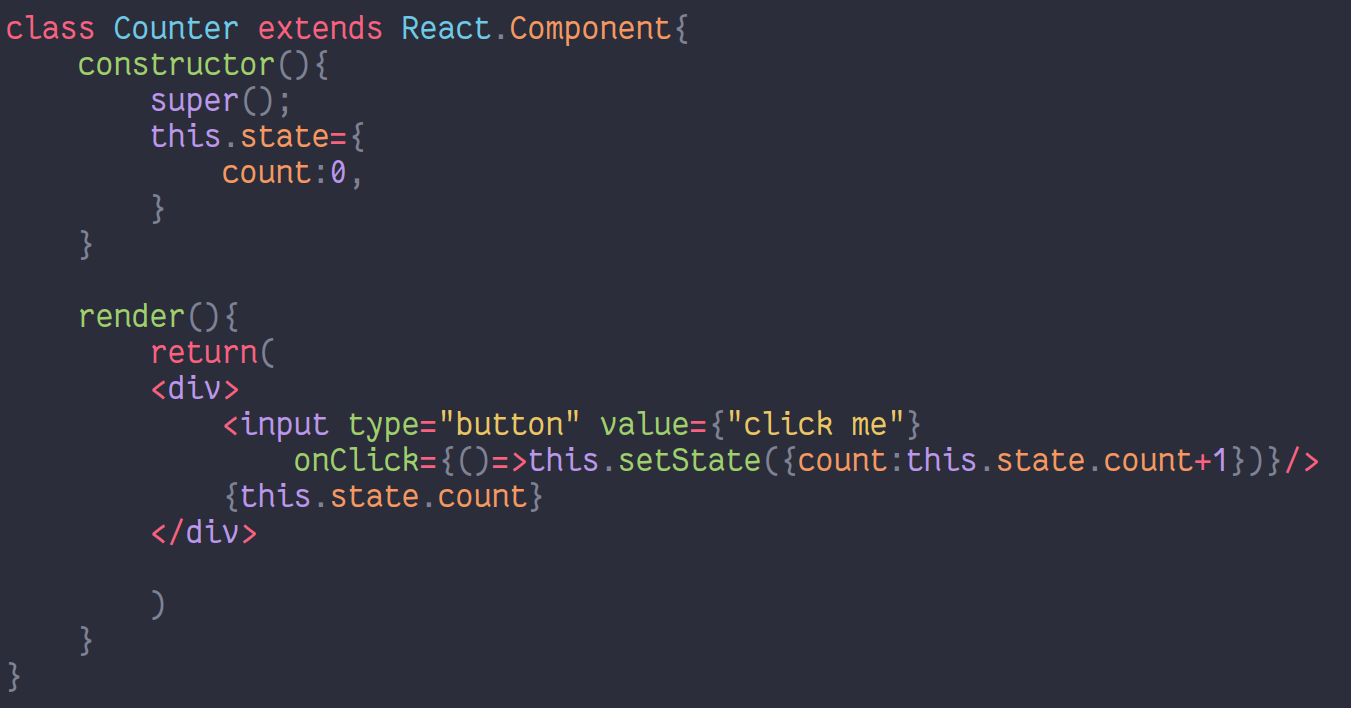
\includegraphics[width=15cm]{src/public/oppar/class_.png}\\
Kuva \getImgCount{}. kuvakaappaus React luokkakomponentista(POISTA CURSOR KUVASTA)
\medskip

% get some src for this
% we can prob link the docs if we find the right page

% In the class component of a React application, the state is stored in the this.state property.
% This state can be dynamically modified and updated by using the this.setState function,
% which allows for re-rendering of the component to reflect the changes in the state and ensures that the user interface stays in sync with the underlying data.

% in the class component state is stored in the this.state property and it can be modified by using the this.setState function
Luokkakomponentissa komponentin tilaa säilytetään this.state ominaisuudessa, ja sitä voi muuttaa tai päivittää käyttämällä this.setState funktiolla. 
Funktio uudelleen renderöi osat komponentista jotka ovat riippuvaisia kyseisestä tilasta.
\medskip

%https://react.dev/reference/react/hooks
% 31.5

Funktio componentissa tila hallinnoidaan "React hookeilla"{}. 
"Hookit"{} antavat funktio komponenteille mahdollisuuden käyttää Reactin ominaisuuksia, 
jotka luokkakomponentit saavat kun ne jatkavat Reactin "Component"{} luokkaa.\labcite{react24b}
%
React kehottaa käyttämään funktiokomponentteja. 
%jotenkin paremmin yhdistää nämä
Funktiokomponenteissa on myös vähemmän koodia kun luokka komponentissa vaikka lopputulos on sama\labciteend{react24c}
Kuvan \prevImageCount{} ja {\the\numexpr \theimgCounter - 2}{} komponentit ovat tehty React 18.3.1 versiolla.





\medskip



\subsubsection{DOM ja VDOM}

% ekassa kappaleessa on tosi lyhyitä lauseita joita ei ole yhdistetty
% vikassa kappaleessa on jotain sus

%html esimerkin alla oleva kappale voidaan siirtää sen päälle


%psychotic
% dom ei ole pakko olla puu formaatti se pitää mainita
DOM (eng Document object model) on puu-struktuurinen representaatio HTML dokumentista.
Tätä struktuuria käytetään rajapintana JavaScriptin ja HTML:län välillä. 
Struktuurissa jokainen solmu on objekti, joka esittää osaa dokumentista. 
Soulmuissa voi olla yksi tai useampi objekti ja nämä objektit voivat osoittaa muihin solmuihin.\labcite{w3org}



esimerkiksi dom representaatio seuraavasta html koodista

% https://www.w3.org/TR/WD-DOM/introduction.html
% kuva ja koodi molemmat täältä.. 29.5 viitatti
    
%pitää viitata jotenkin
\begin{tcolorbox}
\begin{lstlisting}[language=html]
<TABLE>
    <ROWS> 
      <TR> 
          <TD>Shady Grove</TD>
          <TD>Aeolian</TD> 
      </TR> 
      <TR>
          <TD>Over the River, Charlie</TD>
          <TD>Dorian</TD> 
      </TR> 
    </ROWS>
</TABLE>
\end{lstlisting}
\end{tcolorbox}


Esimerkki HTML koodissa luomme pöydän, jossa tehdään kaksi riviä ROWS elementin alle. 
%sisältää väärä sana
Joka riviin tulee kaksi "table data"{} elementtiä, jotka sisältää datan tekstinä.
% mainitse allaoleva kuva tässä
kuvassa \nextImageCount {} HTML on muotoiltu DOM puuhun.
\bigskip



%kuva html domista
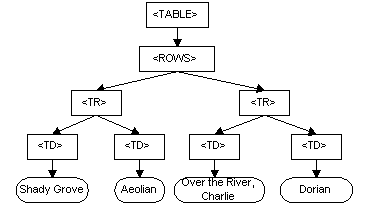
\includegraphics{./src/public/oppar/dom.png}

Kuva\getImgCount .{} DOM puu esimerkki HTML koodista. \labcite{w3org}
\medskip


% en tiedä puuttuuko jotain kappaleesta

DOM toimii rajapintana HTML ja XML dokumentteihin.\labcite{w3org}
Päivityksien tekeminen DOM rajapintaa käyttäen on helppoa, mutta se tulee suorituskyvyn hinnalla.
Elementin päivittäminen DOM:issa päivittää kyseisen elementin kaikki lapsi elementit. 
Tästä päivityksestä voi tulla hyvin kallis, jos elementtejä on paljon.\labcite{refine23}

\bigskip




Käyttöliittymä päivityksien nopeuttamiseksi React on ottanut käyttöön VDOM:in (eng virtual DOM).
VDOM on virtuaalinen esitys DOM:ista, jonka react pitää musitissaan koko suorituksen ajan\labciteend{refine23}
% tekee, se tekee uusiks
Kaikki käyttöliittymä päivitykset mitkä React tekee, se tekee ne VDOM:iin.
Kun muutoksia tapahtuu VDOM:issa niin uusi VDOM puu luodaan. React sitten määrittää mitkä komponentit ovat muuttuneet, erottelu prosessilla (eng diffing).
Erottelu prosessin ansiosta React tietää mikä on pienin määrä muutoksia mitä pitää tehdä oikeaan DOM:iin että käyttöliittymä pysyisi ajan tasalla.\labcite{bharathkumar23}
Elementtien päivittely yksi kerrallaan jokaisen päivityksen ohessa olisi hidasta,
joten react tekee ensiksi kaikki päivitykset VDOM:iin, jonka jälkeen päivittää oikean DOM:in yhdellä kerralla.\citemissing
\medskip



